%!TEX root = ../report.tex
\documentclass[report.tex]{subfiles}
\begin{document}
    \chapter{State of the Art}
    \label{State of the Art}
    \section{Robot dynamic}
    \noindent A robot manipulator, refers to a mechanical system consisting of a set of rigid bodies call \textit{links} which interconnected by \textit{joints}. These joints facilitate relative motion between neighboring links, granting the manipulator the capability to maneuver in a variety of ways within its workspace. The spatial arrangement of the manipulator's joints and links lead to physical constraint which limits the direction of the motion that is being executed.\\
    The motion of a rigid body, to be precise, the forces and accelerations of a rigid body, are being studied in the field of robot dynamics which encompasses both \textit{forward} and \textit{inverse} dynamics. The motions are described by the dynamic equation which being evaluated by dynamic algorithm which solve the numerical value that related to the dynamics\cite{featherstone2007book}.
    In \textit{forward Dynamic}(FD), an applied force to a rigid body is given to calculate the acceleration respon of such input\cite{featherstone2007book}. The equation of motion of FD is expressed in the following form:
    \begin{align}
            \ddot{q} = H(q)^{-1}(\tau - C(q,\dot{q}))
    \end{align}
    In equation (3.1), $\tau$ is a vector of generalized force in joint space. $q$ , $\dot{q}$ and $\ddot{q}$ are the vector of position, velocity and acceleration in joint space respectively. $H(q)$ is the interia matrix which is a function of $q$. At last, $C(q,\dot{q})$ represent the generalized bias force which comprises Coriolis, centrifugal and gravity forces in joint space with other external force that possibly act on the system\cite{featherstone2007book}.\\
    Conversely, Inverse dynamics (ID) computes the necessary force required to generate a given or desired acceleration within a system of rigid bodies. The equation of motion of ID is expressed in the following form\cite{featherstone2007book}:
    \begin{align}
        \tau  = H(q)\ddot{q}+ C(q,\dot{q})
    \end{align}

    Besides forward dynamic and inverse dynamic, Hybrid Dynamic (HD) contains both dynamic problems by given/known $\tau$ or $\ddot{q}$ of a specific joint to compute the unknown forces and accelerations.\\
    Pratically, as a safer method to visualise the effect of validating the solution of control signal and power consumption,in research and development,researchers and roboticitsts frequently use stimulation to perform experiments and developments before deploying on a physical robot. There are many existing software solutions and libraries provide physics engine solutions for simulating physical interactions and dynamics in robotics. Dynamic Animation and Robotics Toolkit (DART)\cite{Lee2018}, Open Dynamics Engine (ODE)\cite{ODE}, Bullet Real-Time Physics engine\cite{Admin_2022} and MuJoCo (Multi-Joint dynamics with Contact) physics engine\cite{MuJoCo}. The physics engines menntioned above uses numbers of aformentioned dynamic solvers such as The Recursive Newton-Euler Algorithm (RNEA) and Articulated Body Algorithm (ABA).

    % \end{enumerate}
    \section{Dynamic solver}
    This session introduces some common dynamic algorithms that being used to solve the dynamic problem mentioned aforenamedly.
    \raggedbottom
    \paragraph*{\large{The Articulated Body Algorithm (ABA)}\\ }
    The Articulated Body Algorithm (ABA) computes the dynamics and motion of articulated bodies. This algorithm models the dynamics of each body in the system using a hierarchical approach, taking into account the interactions between the bodies and the forces acting upon them. The ABA solver is used to solve a forward dynamics problem, where accelerations are calculated from input torques\cite{featherstone1999divide}. 
    \begin{algorithm}[H]
        \caption{The Articulated Body Algorithm (ABA)\cite{featherstone2007book}}
        \label{alg:ABA}
        $\bm{v_0 = 0}$\\
        \Begin{
            \For{i = 1 to $N_B$}{
                $[\textbf{X}_j,\textbf{S}_i,\bm{v}_J,\bm{c}_J] = $jcalc(jtype($i$),$\bm{q_i}$,$\bm{\dot{q_i}}$)\\
                $^{i}\textbf{X}_{\lambda(i)} = \textbf{X}_J \textbf{X}_T(i)$\\
                \If{$\lambda(i) \neq 0$}{
                $^{i}\textbf{X}_0 = {^{i}\textbf{X}_{\lambda(i)}}^{\lambda(i)}\textbf{X}_0$
                }
                $\bm{v}_i = ^{i}\textbf{X}_{\lambda(i)}{} \bm{v}_{\lambda(i)} + \bm{v}_j$\\
                $\bm{c}_i = \bm{c}_J + \bm{v}_i \times \bm{v}_j$\\
                $\bm{I}_i^A = \bm{I}_i$\\
                $\bm{p}_i^A = \bm{v}_i \times^{*} \bm{I}_i \bm{v}_i - {^{i}X_0^{*}} f_i^x$

            }

            \For{$i=N_b$ to 1}{
              $\bm{U}_i = I_i^A S_i$\\
              $\bm{D}_i = S_i^T U_i$\\
              $\bm{u}_i = \tau_i - \bm{S}_i^T \bm{p}_i^A$\\
              \If{$\lambda(i) \neq 0$}{
                $\bm{I}^a = \bm{I}_i^A -\bm{U}_i \bm{D}_i^{-1} \bm{U}_i^T$\\
                $\bm{p}^a = \bm{p}_i^A + \bm{I}^a \bm{c}_i + \bm{U}_i \bm{D}_i^{-1} \bm{u}_i$\\
                $\bm{I}_{\lambda(i)}^A = \bm{I}_{\lambda(i)}^A + {^{\lambda(i)}\bm{X}_i^*} \bm{I}^a {^i\bm{X}_{\lambda(i)}}$\\
                $\bm{p}_{\lambda(i)}^A = \bm{p}_{\lambda(i)}^A + {^{\lambda(i)}\bm{X}_i^*} \bm{p}^a$
              }
            }
            $\bm{a}_0 = -\bm{a}_g$\\
            \For{i = 1 to $N_B$}{
                $\bm{a^{'}} = {^i\bm{X}_{\lambda(i)}} a_{\lambda(i)} + \bm{c}_i$\\
                $\bm{\ddot{q}_i} = \bm{D}_i^{-1}(\bm{u}_i - \bm{U}^T\bm{a}^{'})$\\
                $\bm{a}_i = \bm{a^{'}} + \bm{S}_i \bm{\ddot{q}}_i$\\
            }
        }
    \end{algorithm}
    In the context of the Articulated Body Algorithm (ABA) and a robot with 6 degrees of freedom (DOF), ABA does not support the definition of partial task specifications for bias forces that are not represented as a 6x1 vector. As an illustration, consider the scenario where we aim to define a bias force along the linear z-direction, which naturally arises from forces like gravity. Achieving this particular specification can prove challenging within the Articulated Body Algorithm (ABA) because, in a 6x1 vector, we can only assign a zero value to such a direction. However, merely setting a value to zero does not faithfully replicate the motion dictated by nature.
    In contrast, the Popov-Vereshchagin hybrid solver offers a solution. As outlined in Chapter \ref{Task interfaces}, it allows for the assignment of a 5x1 vector, enabling partial specification and providing the flexibility to accurately capture the desired behavior.
    \raggedbottom
    \paragraph*{\large{The Recursive Newton-Euler Algorithm (RNEA)}\\}
    The Recursive Newton-Euler Algorithm (RNEA) is a recursive approach to solving the inverse dynamics problem, which involves calculating joint-space torques from joint-space accelerations for each body in a system. This algorithm takes into account the relationships between the bodies and the forces acting upon them. It is aimed to streamline and improve the computation of dynamics in complex multi-segmented robot manipulator. The recursive approach minimizes repetitive calculations and boosts computational effectiveness.Featherstone's book illustrate the algorithm as follow:\cite{featherstone2007book}.\\
    \begin{algorithm}[H]
        \caption{The Recursive Newton-Euler Algorithm (RNEA)}
        \label{alg:ALG1}
        $\bm{v_0 = 0}$\\
        $\bm{a_0 = 0}$\\
        \Begin{
            \For{i = 1 to $N_B$}{
                $[\textbf{X}_j,\textbf{S}_i,\bm{v}_J,\bm{c}_J] = $jcalc(jtype($i$),$\bm{q_i}$,$\bm{\dot{q_i}}$)\\
                $^{i}\textbf{X}_{\lambda(i)} = \textbf{X}_J \textbf{X}_T(i)$\\
                \If{$\lambda(i) \neq 0$}{
                $^{i}\textbf{X}_0 = ^{i}\textbf{X}_{\lambda(i)}{}^{\lambda(i)}\textbf{X}_0$
                }
                $\bm{v}_i = ^{i}\textbf{X}_{\lambda(i)}{} \bm{v}_{\lambda(i)} + \bm{v}_j$\\
                $\bm{a}_i = ^{i}\textbf{X}_{\lambda(i)}{} \bm{a}_{\lambda(i)} + \textbf{S}_i \ddot{q_i}+ \bm{c}_J+\bm{v}_i\times \bm{v}_J$\\
                $\bm{f}_i = \textit{\textbf{I}}_i \bm{a}_i+\bm{v}_i\times^{\ast}\textit{\textbf{I}}_i \bm{v}_i - ^{i}\textbf{X}_0^\ast \bm{f}_i^x$
            }

            \For{$i=N_b$ to 1}{
                $\tau_i = \bm{S}^T_i \bm{f}_i$\\
                \If{$\lambda(i) \neq 0$}{
                $\bm{f}_{\lambda(i)} = \bm{f}_{\lambda(i)}+ ^{\lambda(i)}\textbf{X}_i^\ast \bm{f}_i^x$
                }
            }
        }
    \end{algorithm}
    Notice on line 11, the algorithm takes $\ddot{q_i}$ as input to compute $a_i$. However when we input a task specification or constraint $\ddot{\bm{X_}N}$, we need to map the task specification in Cartesian space $\ddot{\bm{X_}N}$ to joint space $\ddot{q_i}$ with:
    \begin{align}
        \ddot{\bm{X_}N} &= \bm{J}_N \ddot{q}\\
        \label{eq:q_jac} \ddot{q} &= \bm{J}_N^{-1} \ddot{\bm{X_}N}
    \end{align}
    From \ref{eq:q_jac} , $\ddot{\bm{X_}N}$ requires task specification in all 6 directions which lead to lacking flexibility of giving partical task specification. However,  Popov-Vereshchagin hybrid solver resolves this issues by allowing partical task specification. A details explaination of different task specification will be discussed in chapter \ref{Background} section \ref{Task interfaces}.
    \raggedbottom
    \paragraph*{\large{The Articulated-Body Hybrid Dynamics Algorithm (ACHDA)}\\}
    The Articulated-Body Hybrid Dynamics Algorithm (ACHDA) is capable of computing three types of dynamics: inverse dynamics, forward dynamics, and hybrid dynamics. In inverse dynamics, the solver calculates joint torques from Cartesian acceleration constraints. In forward dynamics, the solver takes feed-forward joint torques as input and computes Cartesian accelerations. In hybrid dynamics, the solver combines both of the above methods. Additionally, as a byproduct, it can also take external forces as input and compute joint accelerations.\cite{featherstone2007book}.

    \section{Controller}
    \label{Controller}
    Controller guides systems toward desired setpoints or references value with feeback loop. The followings are some common controllers that are widely used in rocotics.
    \paragraph*{\large{Proportional-integral-derivative (PID) controllers}\\}
    Proportional-Integral-Derivative (PID) controllers uphold a specific setpoint. In this R\&D project, PID controller regulates position and velocity by using the equation below:
    \begin{align}
        u(t) = K_pe(t) + K_i\sum_{t=0}^{t} e(t) \Delta{t} + K_d \frac{e(t)-e(t-1)}{\Delta{t}}
    \end{align}
    Where $u(t)$ is the control signal at time $t$. $e(t)$ is the error at time $t$ as the difference between the setpoint and the current input of the controller. $\Delta{t}$ is the time step of each calculation in the control loop. $K_p$, $K_i$, $K_d$ are the coefficients of proportional, integral and derivative gain respectively\cite{johnson2005pid}.

    \paragraph*{\large{Fuzzy logic algorithm}\\}
    Fuzzy logic algorithms employed as controllers adeptly navigate scenarios marked by uncertainty, adeptly utilizing linguistic terms and membership functions to accurately represent the gamut of inputs and outputs. This approach hinges upon rule-based decision-making, whereby the system gauges the extent of each rule's applicability contingent upon the values presented in the input domain \cite{dadios2012fuzzy}.
    \paragraph*{\large{Impedance controllers}\\}
    Impedance controller emulate the the mechanical properties of stiffness and damping to regulate the forces and motions relationship when the robot interacts with objects. Extend from equation (3.2) with two main components: Stiffness and Damping Component. A basic Impedance controller is formed.
    \begin{align}
            \tau  = K(q_d -q) + D (\dot{q_d} - \dot{q}) + H(q)\ddot{q}+ C(q,\dot{q})
    \end{align}
    Where $K$ and $D$ are stiffness-like and damping-like matrix, respectively \cite{song2017impedance}.
    \section{Task based control}
    Task-based control in robotics refers to a control approach that focuses on achieving specific tasks or objectives rather than directly controlling individual joints or degrees of freedom. Instead of commanding the robot's joints to move in a prescribed manner, task-based control involves specifying the desired behaviors or goals the robot should accomplish.
    \paragraph*{\large{iTaSC}\\}
    iTaSC is a control framework that was introduced by \cite{smits2008itasc}. It is the fusion of instantaneous task specification and estimation of geometric uncertainty that focuses on achieving tasks while respecting various constraints. These constraints could include safety considerations, physical limitations, interaction forces, and more. The framework provides a way to dynamically adjust a robot's behavior in real time, allowing it to respond to changing conditions and maintain safe and effective interactions with the environment. Later \cite{decre2009extending} extended the idea of iTaSC.\\
    In a multi-sensor robot system, a task is described as the desired behaviors or objectives that the robot needs to achieve. These tasks are formulated in the task space, which represents the robot's end-effector or operational space. The tasks and constraints had to be formulated at the begining. Task formulation encompasses goal position, following a particular trajectory or maintaining a certain force. constraint formulation contains obeying joint limits, velocity limits ,avoiding collisions. etc. Based on their priorities,tasks and constraints are organized in a hierarchical manner. Two set of coordinates were introduced to represent the tasks and constraints, feature and uncertainty coordinate. Feature coordinate expresses the relative mottions between feature on the specific obejcts. uncertainty coordinate represent geometric uncertainties.\\
    The authers proposed general control and estimation scheme:
    \begin{figure}[h!]
        \centering
        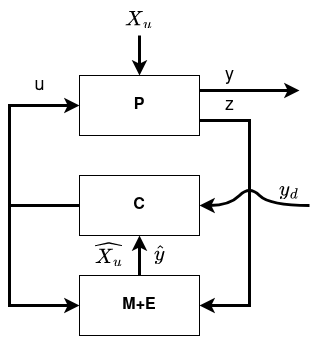
\includegraphics[width=0.4\linewidth]{images/iTaSC.png}
        \caption{A general control and estimation scheme.\cite{smits2008itasc}}
        \label{fig:itasc}
    \end{figure}
    Where the robot system and the environment are are denoted as \textit{plant} P which observer the senser measurements $z$. $u$is the control input (joint posiitons,velocities and torques) that compute from controller $C$. Contoller takes the estimates $X_u$ and $\widehat{y}$ as input where both of them are generated from \textit{Model Update and Estimation block} M+E  estimate $\widehat{y}$ which takes the controlled input signal $u$ and measurements $z$ as input to estimate $y$ as the output of the system.\\
    Later, \cite{vanthienen2013force} poposed using iTaSC on force-sensorless robot force control. Figure \ref{fig:itasc_nosensor} show the one degree-of-freedom (DOF) robot force control scheme that can extend to mult degree-of-freedom scenerio.\\
    \begin{figure}[h!]
        \centering
        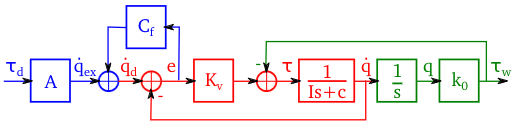
\includegraphics[width=0.8\linewidth]{images/iTaSC_nosensor.png}
        \caption{One degree-of-freedom robot force control scheme.\cite{vanthienen2013force}}
        \label{fig:itasc_nosensor}
    \end{figure}\\
    In figure \ref{fig:itasc_nosensor}, the robot system model and the underlying joint velocity controller are depicted in red. The stiffness model pertaining to environmental contact is showcased in green, while the controller section open to design is highlighted in blue. The gravity term is omitted because the robot was being used in the experiment was gravity-compensated mechanically. This is a first order system with a desired input $\tau_d$ and output $\dot{q}$ in non-contact situation. In contrast,the green part is included. The model characterizes a second-order system where $\tau_d$ serves as the input, and the resulting torque $\tau_w$ exerted on the environment acts as the output. The joint velocity error feedback constant, $C_f$, results in the modification of the velocity loop feedback constant $K_v$, leading to an equated velocity loop feedback constant $\frac{K_v}{1-C_f}$. In mult degree-of-freedom scenerio, all the previously mentioned variables becomes vector and the constants becomes matrices \cite{vanthienen2013force}.

    \paragraph*{\large{Stack of tasks}\\}
    The paper from \cite{mansard2009unified} and \cite{mansard2009versatile} introduced Stack of tasks (SoT) which provides a way to manage multiple objectives and constraints in a coherent and organized manner. It ensures that the robot's control algorithm focuses on achieving the most critical tasks first while considering the constraints and interactions among tasks and generalized the concept of hierarchy-based control strategies to include unilateral constraints at various levels of priority.
    \section{Existing implementation of exploting surface in robot manipulation}\label{Existing implementation of exploting surface in robot manipulation}
    There were some existing implementation or discussion about exploting surface in robot manipulation. In \cite{salvietti2015modeling} ,authors presented a mathematical framework that outlines the interaction between compliant hands and environmental constraints during the execution of a grasping task. \cite{eppner2015planning} discussed planning grasp strategies that exploit environmental constraints. In this paper, each environmental constraint exploitation is considered as one controller with a desired spatial and contact condition with a termination predicate which is also a switching condition if the constraint is in between the motion in global point of view. The final motion planing consists of a series of environmental exploits that lead to a grasp.
    \section{Limitations of previous work}\label{Limitations of previous work}
    In today's world, there's an ongoing challenge in deciding between investing in an expensive, lightweight robot arm or a more affordable but heavier one. This decision-making is influenced by limited financial resources for development. Opting for cheaper, heavier robots can lead to smoother but less precise robotic movements, affecting accuracy.\\Interestingly, current robot motion planning still treats contact surfaces as obstacles to be avoided. The well-known dynamic solvers like ABA and RNEA don't handle situations where only some constraints are present very well. As of now, the existing researches relys on visual or other sensory input to detect contact surface. However,there's a lack of research on how to adapt the Vereshchagin solver to scenarios where contact is made by joints other than the end-effector, and how to practically implement this idea without including sensors on the robot.
\end{document}